\documentclass[conference]{IEEEtran}
\IEEEoverridecommandlockouts

\usepackage{cite}
\usepackage{amsmath,amssymb,amsfonts}
\usepackage{graphicx}
\usepackage{textcomp}
\usepackage{xcolor}
\usepackage{booktabs}
\usepackage{multirow}
\usepackage{hyperref}

\graphicspath{{figures/}}

\begin{document}

\title{Temporal Modeling vs.\ Structured Preprocessing:\\
A Controlled Comparison for Early Sepsis Prediction}

\author{
  \IEEEauthorblockN{George Arthur}
  \IEEEauthorblockA{CS6140 Machine Learning\\
  Northeastern University\\
  Boston, MA, USA}
}

\maketitle

% Abstract
\begin{abstract}
Early prediction of sepsis in the intensive care unit (ICU) is a critical clinical
challenge, where timely intervention can significantly reduce mortality. This paper
investigates whether temporal sequence modeling (LSTM) or structured preprocessing
(missingness-aware feature engineering) is the stronger lever for improving early
sepsis prediction. Using the PhysioNet/CinC 2019 dataset of 40,336 ICU patients,
we conduct a controlled 2$\times$2 experiment across two preprocessing strategies
(median imputation vs.\ forward-fill with missingness indicators) and two model
families (XGBoost and LSTM). Results show that XGBoost with missingness-aware
preprocessing (AUPRC\,=\,0.1730, 95\% CI [0.1636, 0.1825]) consistently outperforms
LSTM across both strategies, and that preprocessing choice is the dominant factor.
SHAP analysis reveals ICULOS, hospital admission time, and respiratory trends as
the most predictive features. The best model generalises reasonably across two
hospital systems (Set A AUPRC\,=\,0.1824, Set B\,=\,0.1625).
\end{abstract}

\begin{IEEEkeywords}
sepsis prediction, ICU, XGBoost, LSTM, missingness indicators, SHAP, PhysioNet
\end{IEEEkeywords}

% I. Introduction
\section{Introduction}

Sepsis, defined as life-threatening organ dysfunction caused by dysregulated host
response to infection \cite{singer2016third}, affects over 1.7 million adults
annually in the United States and carries a mortality rate of 15--30\%. Early
detection remains difficult: sepsis progresses rapidly, its onset is diffuse, and
clinical features overlap with other conditions. Automated early-warning systems
that operate on routinely collected ICU data offer a promising path to earlier
intervention.

Two broad approaches dominate the literature. The first relies on temporal sequence
models such as LSTMs \cite{hochreiter1997long} to capture complex dependencies
across time. The second focuses on feature engineering, particularly on how
missing values are handled, to extract more signal from sparse, irregularly sampled
clinical measurements. In practice, ICU lab values can be missing for 60--80\% of
timesteps \cite{harutyunyan2019multitask}, making missing data treatment a first-order
methodological choice.

This paper poses a simple question: \textit{which matters more, temporal model
architecture or preprocessing strategy?} We answer this through a controlled
2$\times$2 experiment on the PhysioNet/CinC 2019 sepsis dataset \cite{reyna2019early},
crossing two preprocessing strategies with two model families.

% II. Dataset
\section{Dataset and Experimental Setup}

\subsection{PhysioNet/CinC 2019 Dataset}

The dataset comprises 40,336 ICU patients from two hospital systems (Set A: 20,336;
Set B: 20,000), each represented as an hourly time series of 40 clinical features:
8 vital signs, 26 laboratory values, and 6 demographic variables. The original
\texttt{SepsisLabel} is a binary indicator shifted 6 hours before clinical onset to
create an early-warning target (\texttt{EarlyLabel}). Patients with sepsis onset
within the first 6 hours (706 patients) were excluded as no valid prediction window
exists. The final cohort (39,630 patients, 5.62\% sepsis prevalence) was split
70/15/15 into stratified patient-level train/validation/test sets, preserving class
prevalence across all splits.

\subsection{2$\times$2 Experimental Design}

We define four conditions as the Cartesian product of two preprocessing strategies
and two model families:

\begin{itemize}
  \item \textbf{Strategy A}: Median imputation (per-feature training median) followed
        by standard scaling. Simple and widely used.
  \item \textbf{Strategy B}: Per-patient forward-fill of the last observed value,
        supplemented by binary missingness indicator columns for each of the 40
        original features. This encodes \textit{when} values were missing as an
        explicit signal \cite{rubin1976inference,che2018recurrent}.
\end{itemize}

For XGBoost (Conditions A and B), 48 lag features were added per condition:
6 temporal statistics (lag-1, lag-2, lag-4, 4-hour rolling mean/std, 1-hour delta)
for each of the 8 vital signs, applied after the patient-level split to prevent
data leakage. Final feature counts: Condition A (88 features), Condition B (125
features). For LSTM (Conditions C and D), raw time series of 40 features (Strategy A)
or 76 features (Strategy B) were fed as padded sequences up to 72 timesteps.

% III. Methods
\section{Methods}

\subsection{XGBoost}

XGBoost \cite{chen2016xgboost} was trained with \texttt{scale\_pos\_weight\,=\,43.3}
to account for the 43:1 class imbalance. Hyperparameters were selected via grid
search over \{3, 4, 6\} tree depths and \{0.05, 0.1\} learning rates, with 500
estimators and early stopping (patience 20) on validation AUPRC.

\subsection{LSTM}

A two-layer LSTM \cite{hochreiter1997long} with a per-timestep linear output head
was implemented in PyTorch \cite{paszke2019pytorch}. Packed padded sequences
handled variable-length patient stays. Training used BCEWithLogitsLoss with
\texttt{pos\_weight\,=\,43.3}, Adam optimiser, gradient clipping
(\texttt{max\_norm\,=\,1.0}), and early stopping (patience 10). Grid search covered
hidden sizes \{64, 128\}, dropout rates \{0.2, 0.3\}, and learning rates
\{0.001, 0.0005\}.

\subsection{Evaluation}

The primary metric is AUPRC (Area Under the Precision-Recall Curve), which is robust
to class imbalance and directly reflects the precision-recall trade-off relevant to
clinical screening. AUC-ROC is reported as a secondary metric. Metrics were computed
using scikit-learn \cite{pedregosa2011scikit}. Decision thresholds were selected by
maximising F1 on the validation set. All reported metrics are accompanied by 95\%
bootstrap confidence intervals (1,000 iterations, patient-level resampling). SHAP
TreeExplainer \cite{lundberg2017unified} was applied to both XGBoost models to assess
feature importance.

% IV. Results
\section{Results}

\subsection{Main Results}

Table~\ref{tab:results} presents the full 2$\times$2 comparison. XGBoost with
Strategy B (Condition B) achieves the highest test AUPRC of 0.1730 (95\% CI
[0.1636, 0.1825]), representing a 7.5$\times$ improvement over the random baseline
(prevalence\,=\,0.023). Both LSTM conditions perform substantially below their
XGBoost counterparts, with Condition C (AUPRC\,=\,0.0625) and Condition D
(AUPRC\,=\,0.0618) showing no meaningful benefit from the richer Strategy B
preprocessing.

\begin{table}[h]
\centering
\caption{2$\times$2 Experimental Results (Test Set)}
\label{tab:results}
\begin{tabular}{llccc}
\toprule
\textbf{Cond.} & \textbf{Model} & \textbf{Strategy} & \textbf{AUPRC (95\% CI)} & \textbf{AUC-ROC} \\
\midrule
A & XGBoost & A & 0.1672 [0.158, 0.176] & 0.8325 \\
B & XGBoost & B & \textbf{0.1730} [0.164, 0.183] & \textbf{0.8539} \\
C & LSTM    & A & 0.0625 [0.058, 0.068] & 0.7599 \\
D & LSTM    & B & 0.0618 [0.056, 0.067] & 0.7597 \\
\bottomrule
\end{tabular}
\end{table}

Fig.~\ref{fig:results} shows the AUPRC bar chart with confidence intervals and
precision-recall curves for all four conditions. The non-overlapping confidence
intervals between XGBoost and LSTM conditions confirm that the performance gap is
statistically meaningful.

\begin{figure}[h]
  \centering
  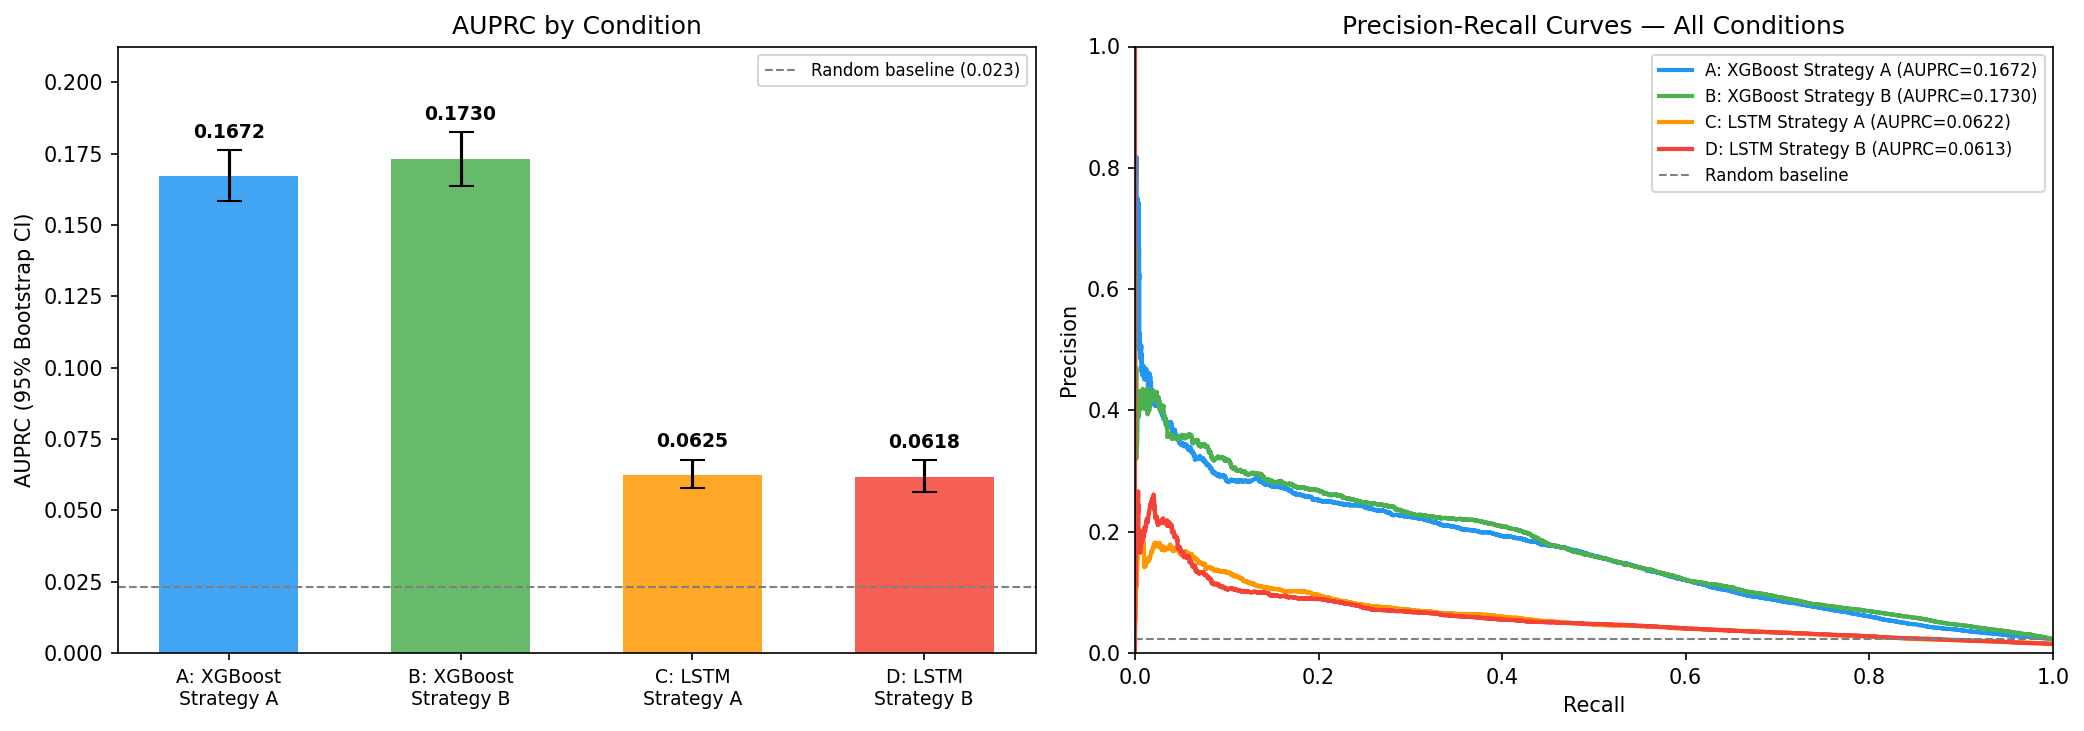
\includegraphics[width=\columnwidth]{results_comparison.png}
  \caption{AUPRC comparison with 95\% bootstrap CIs (left) and
           precision-recall curves (right) for all four conditions.
           Dashed line indicates random baseline (prevalence\,=\,0.023).}
  \label{fig:results}
\end{figure}

\subsection{ROC and Calibration Analysis}

Fig.~\ref{fig:roc_cal} presents ROC curves and calibration plots. Both XGBoost
conditions achieve AUC-ROC above 0.83, while LSTM conditions cluster around 0.76.
Calibration analysis reveals that XGBoost models produce well-calibrated probability
estimates (predicted risk scores track actual event rates closely), whereas LSTM
models are poorly calibrated, producing compressed probability outputs near zero.
This has direct clinical implications: XGBoost risk scores are more suitable for
threshold-based alerting systems.

\begin{figure}[h]
  \centering
  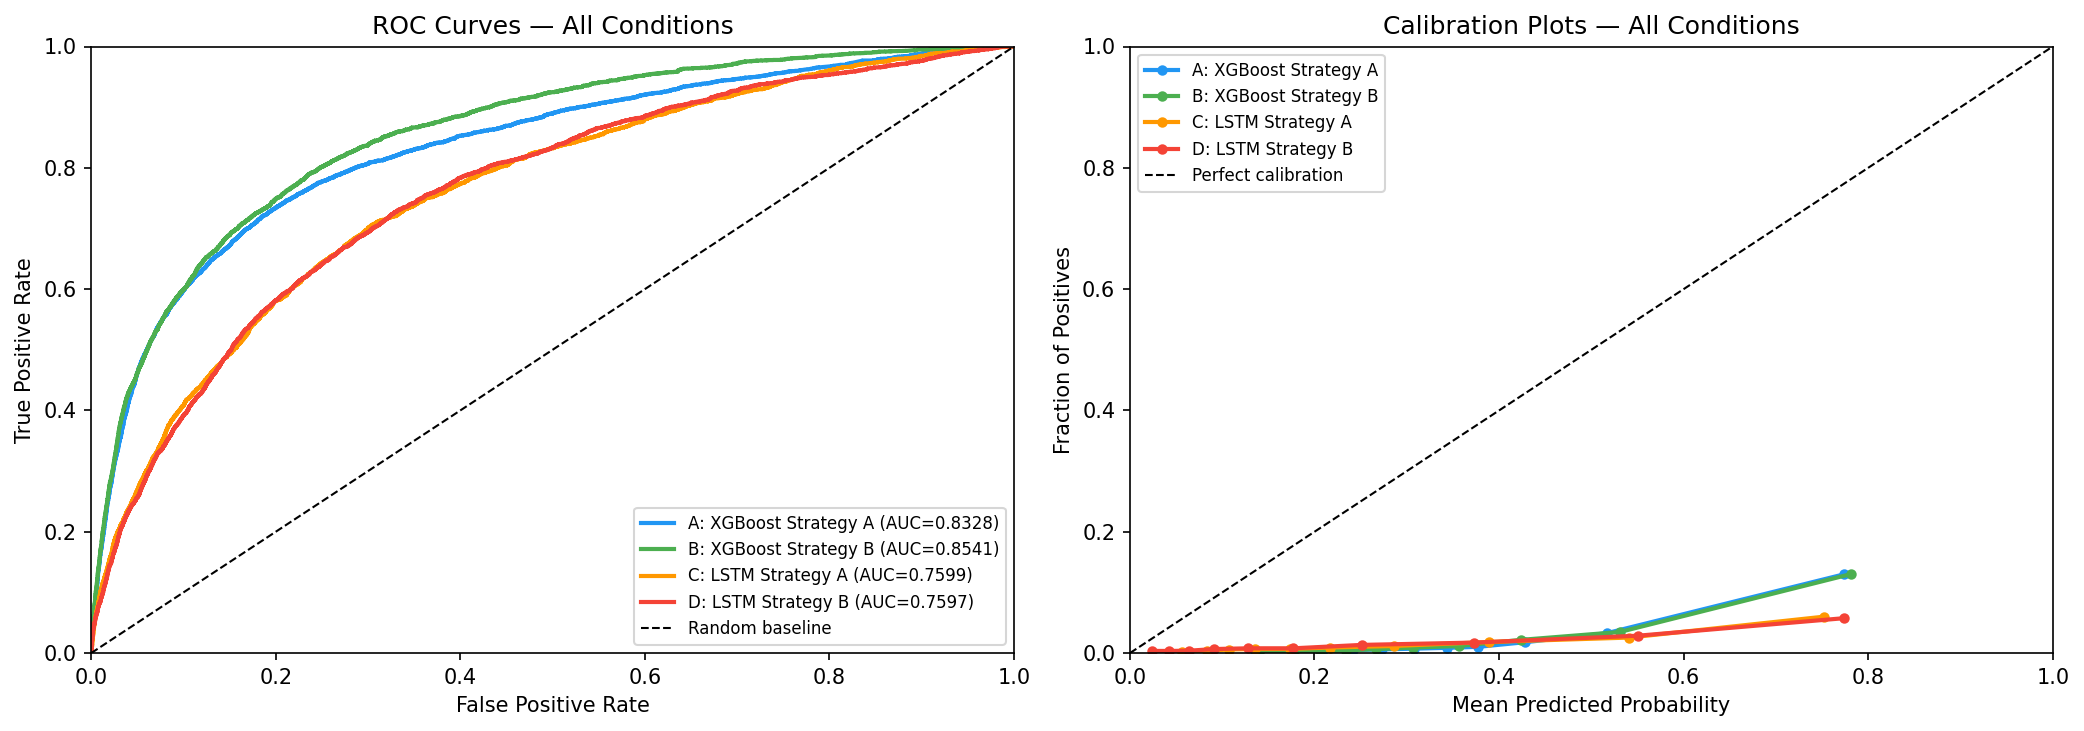
\includegraphics[width=\columnwidth]{roc_calibration.png}
  \caption{ROC curves (left) and calibration plots (right). XGBoost models
           are better calibrated than LSTM models, making their predicted
           probabilities more reliable for clinical decision support.}
  \label{fig:roc_cal}
\end{figure}

\subsection{Feature Importance via SHAP}

Fig.~\ref{fig:shap} shows the top 20 features by mean absolute SHAP value for
Conditions A and B. ICU length of stay (\texttt{ICULOS}) is the dominant predictor
in both conditions, followed by hospital admission time and respiratory rate rolling
mean, capturing the clinical reality that deteriorating respiratory patterns
precede sepsis onset. In Condition B, missingness indicators for FiO$_2$ and EtCO$_2$
appear in the top 20, confirming that the absence of certain measurements carries
genuine clinical signal: physicians may not order these tests when patients are
stable, making their absence informative.

\begin{figure}[h]
  \centering
  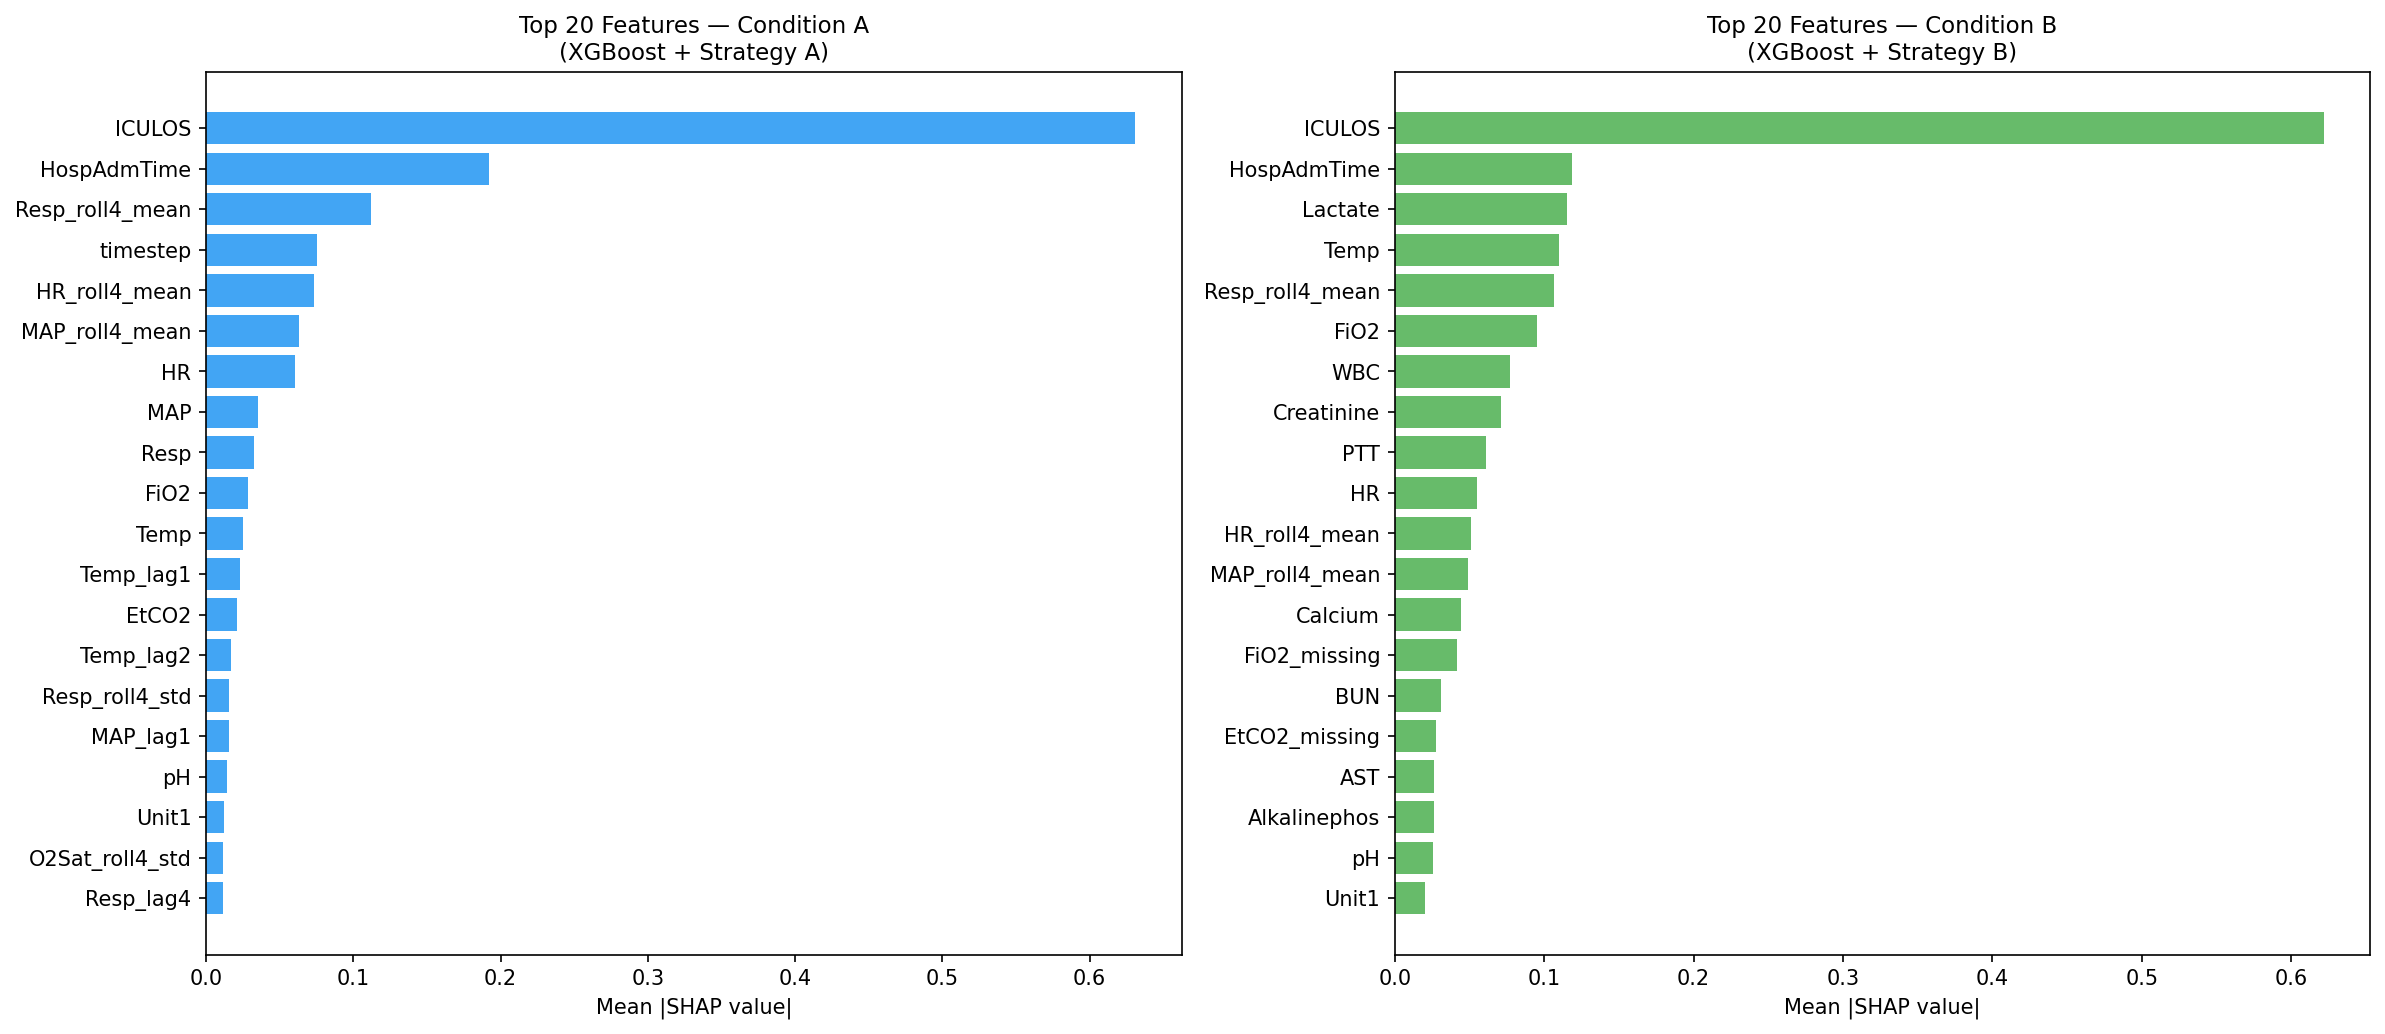
\includegraphics[width=\columnwidth]{shap_top_features.png}
  \caption{Top 20 features by mean $|$SHAP value$|$ for Condition A (left)
           and Condition B (right). Missingness indicators appear in
           Condition B, confirming their predictive value.}
  \label{fig:shap}
\end{figure}

\subsection{Hospital Generalizability}

Fig.~\ref{fig:hospital} shows XGBoost B performance stratified by hospital system.
AUC-ROC is nearly identical (Set A: 0.8504, Set B: 0.8391), indicating that the
model's discriminative ability generalises across institutions. AUPRC shows a modest
gap (Set A: 0.1824, Set B: 0.1625), likely attributable to differences in lab
measurement practices and patient population between hospital systems.

\begin{figure}[h]
  \centering
  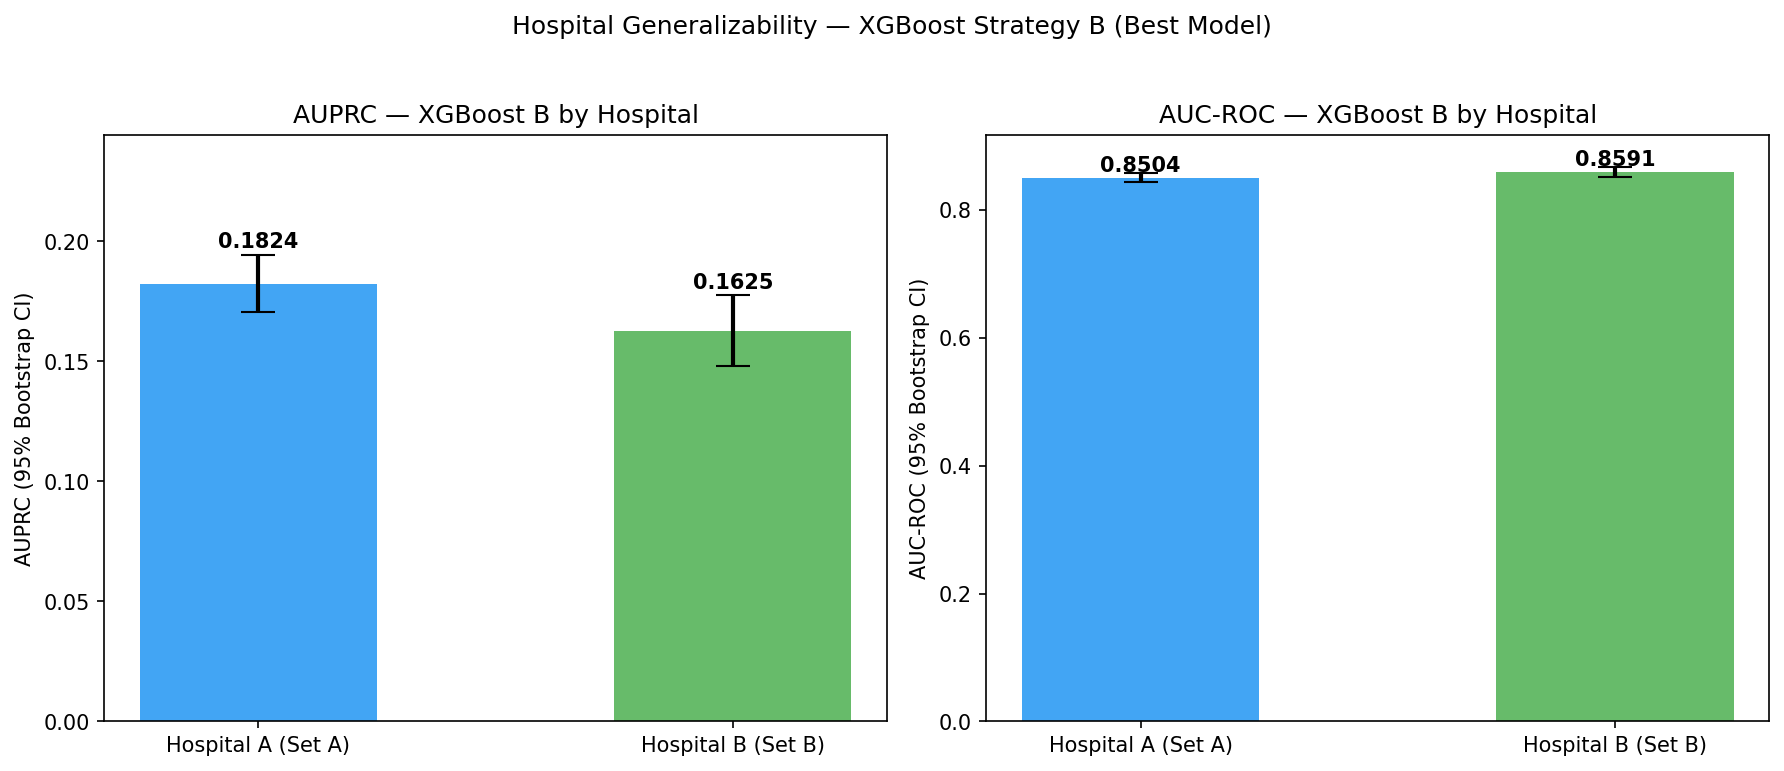
\includegraphics[width=\columnwidth]{hospital_generalizability.png}
  \caption{XGBoost B performance on Hospital Set A vs.\ Set B test patients.
           AUC-ROC generalises well; AUPRC shows modest site-level variation.}
  \label{fig:hospital}
\end{figure}

% V. Discussion
\section{Discussion}

\subsection{Why XGBoost Outperforms LSTM}

The consistent superiority of XGBoost over LSTM on this dataset is explained by
three dataset characteristics. First, ICU lab values are missing for 60--80\% of
timesteps: the sequences seen by the LSTM are largely imputed or forward-filled
values rather than true observations. Second, the 43:1 class imbalance means that
positive timesteps are heavily diluted within each sequence, making it difficult for
the LSTM to identify the relevant signal window. Third, XGBoost's per-timestep
treatment of the data, combined with explicit lag features, effectively captures
temporal dynamics without requiring the model to learn sequential dependencies from
sparse sequences. These findings align with prior work showing gradient boosting
outperforms sequence models on irregular clinical tabular data
\cite{harutyunyan2019multitask}.

\subsection{The Role of Preprocessing}

Strategy B improves XGBoost (AUPRC: 0.1672 $\to$ 0.1730); the confidence intervals
partially overlap (A: [0.1582, 0.1761], B: [0.1636, 0.1825]), so this difference
should be interpreted cautiously. By contrast, the gap between XGBoost and LSTM
conditions is clearly non-overlapping and unambiguous. Strategy B has no meaningful
effect on LSTM performance (0.0625 $\to$ 0.0618). This asymmetry reveals that the
benefit of missingness-aware preprocessing is model-dependent: XGBoost can exploit
missingness indicators as discrete features, while the LSTM's sequence-level
optimisation cannot effectively leverage the same information across largely-missing
sequences.

% VI. Limitations
\section{Limitations and Conclusion}

\subsection{Limitations}

This study has several limitations. The LSTM architecture used is a standard
many-to-many design; architectures specifically designed for irregular time series,
such as GRU-D \cite{che2018recurrent}, may close the performance gap by learning
feature-specific decay rates for missing values. The lag feature engineering for
XGBoost was limited to 8 vital signs; extending to lab values could further improve
performance. Finally, while hospital generalizability is assessed at the test-set
level, prospective validation across additional institutions remains necessary before
clinical deployment.

\subsection{Conclusion}

We conducted a controlled 2$\times$2 experiment comparing preprocessing strategy and
model architecture for early sepsis prediction. XGBoost with missingness-aware
preprocessing achieves the best performance (AUPRC\,=\,0.1730), outperforming
LSTM across both strategies. Preprocessing strategy is the dominant factor for
XGBoost, while LSTM performance is largely insensitive to preprocessing, suggesting
that the limiting factor for sequence models on this dataset is not feature
representation but model-data alignment. Future work should explore architectures
designed for irregular clinical time series and multi-site prospective validation.

% References
\bibliographystyle{IEEEtran}
\bibliography{references}

\end{document}
